\chapter{动态规划(1)}

\begin{introduction}
  \item 带权区间调度
  \item 矩阵链乘法
\end{introduction}

\section{概述}
在前面的课程中,已经学习过了贪心法和分治法两种策略,本章将开始动态规划(Dynamic programming)的学习。
简要比较一下几种算法策略的不同。

\begin{itemize}
  \item 贪心法 -基于贪心策略,每次总是选取眼前最优的选项,同时期待最终的结果最优。
        优点在于思考和模型建立较为简单,难点在于如何证明算法的正确性。
  \item 分治法 -分而治之,子问题不存在重叠。
        难点在于如何分割问题,以及如何合并解。
  \item 动态规划 -思想类似于分治,与贪心法相反,子问题之间存在重叠,算法执行过程中记录子问题的解。
        难点在于如何找到转移方程。
\end{itemize}

本章将介绍动态规划在带权区间调度~\ref{sec:weighted-interval-scheduling} 、矩阵链乘法~\ref{sec:matrix-chain-multiplication} 两个问题上的应用。

\section{带权区间调度}\label{sec:weighted-interval-scheduling}

\subsection{问题描述}

\begin{figure}[hbt!]
  \centering
  \begin{tikzpicture}
    \draw[|-|] (0, 5) -- node [above] {$w_1=2$} (2, 5);
    \draw[|-|] (1, 4) -- node [above] {$w_2=4$} (5, 4);
    \draw[|-|] (3, 3) -- node [above] {$w_3=4$} (7, 3);
    \draw[|-|] (1.5, 2) -- node [above] {$w_4=7$} (8.5, 2);
    \draw[|-|] (8, 1) -- node [above] {$w_5=2$} (10, 1);
    \draw[|-|] (9.5, 0) -- node [above] {$w_6=1$} (10.5, 0);
  \end{tikzpicture}
  \caption{区间调度示例}\label{fig:wis-picture-1}
\end{figure}

下面给出带权区间调度问题的定义。

\begin{definition}{带权区间调度问题}{def:weighted-interval-scheduling}
  给定区间$I_1, I_2, \ldots, I_n$,
  $s_i$为$I_i$开始时间,$f_i$为$I_i$的结束时间($f_i>s_i$),$w_i>0$, 假设$\forall i < j$,$ s_i<s_j$。
  \begin{itemize}
    \item $OPT(k)$:表示区间集合$\{ I_1, I_2, \ldots , I_i \}$上的最优解权值。
    \item $P(i)$:表示$I_i$的前驱,当$P(i)=j$时,有$f_j=\max\limits_{1 \leq k < i}\{f_k | f_k < s_i\}$,当$I_i$没有前驱时,$P(i)=0$
  \end{itemize}
  目标:寻找一个$\sum w_i$最大的区间子集$R$,满足$\forall I_m,I_n \in R, m < n \text{都有} f_m < s_n$。
\end{definition}

通俗来讲,就是找出一个彼此时间不重叠的区间序列,使得这个序列的权重在所有可能的序列中,权重最大。

\begin{remark}
  以\autoref{fig:wis-picture-1}为例,$P(6)=4, P(5)=3, P(4)=0, P(3)=1, P(2)=0, P(1)=0$
\end{remark}

\subsection{贪心}

\begin{figure}[hbt!]
  \centering
  \begin{subfigure}{.3\textwidth}
    \centering
    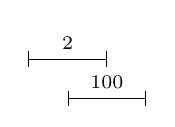
\begin{tikzpicture}
      \draw[|-|] (0, 0) -- node [above] {\scriptsize 2} (1, 0);
      \draw[|-|] (0.5 , -0.5) -- node [above] {\scriptsize 100} (1.5, -0.5);
    \end{tikzpicture}
    \caption{}\label{fig:wis-counterexample1}
  \end{subfigure}
  \begin{subfigure}{.3\textwidth}
    \centering
    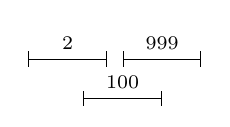
\begin{tikzpicture}
      \draw[|-|] (0, 0) -- node [above] {\scriptsize 2} (1, 0);
      \draw[|-|] (1.2, 0) -- node [above] {\scriptsize 999} (2.2, 0);
      \draw[|-|] (0.7 , -0.5) -- node [above] {\scriptsize 100} (1.7, -0.5);
    \end{tikzpicture}
    \caption{}\label{fig:wis-counterexample2}
  \end{subfigure}
  \begin{subfigure}{.3\textwidth}
    \centering
    \begin{tikzpicture}
      \draw[|-|] (0, 0) -- node [above] {\scriptsize 2} (1, 0);
      \draw[|-|] (1.2, 0) -- node [above] {\scriptsize 3} (2.2, 0);
      \draw[|-|] (0.7 , -0.5) -- node [above] {\scriptsize 6} (1.7, -0.5);
    \end{tikzpicture}
    \caption{}\label{fig:wis-counterexample3}
  \end{subfigure}
  \caption{贪心反例}\label{fig:wis-counterexample}
\end{figure}

\begin{enumerate}
  \item 以最早完成时间排序,反例如\autoref{fig:wis-counterexample1}
  \item 以最大权重排序,反例如\autoref{fig:wis-counterexample2}
  \item 选择冲突最少的区间,反例如\autoref{fig:wis-counterexample3}
\end{enumerate}

常见的贪心思考方向无法解决带权区间调度问题。

\subsection{动态规划}

\subsubsection{算法设计}
观察带权区间调度问题,对于最优解$OPT(n)$,可以得到如下两个结论:
\begin{itemize}
  \item 子集$R$要么包含$I_n$,要么不包含$I_n$
  \item 对于区间$I_n$
        \begin{itemize}
          \item 如果$I_n \in R$,$OPT(n)=w_n+OPT(P(n))$
          \item 如果$I_n \notin R$,$OPT(n)=OPT(n-1)$
        \end{itemize}
\end{itemize}

于是我们可以得到该问题的状态转移方程:
\begin{equation}
  OPT(n) = \begin{cases}
    w_n + OPT(P(n)), & I_n \in R    \\
    OPT(n-1),        & I_n \notin R
  \end{cases}
\end{equation}
\par
因为需要找到最大的权值,上式也可以写成
\begin{equation}
  OPT(n)=\max \{w_n+OPT(P(n)),OPT(n-1)\}
\end{equation}

\subsubsection{算法分析}

\paragraph*{时间复杂度}
在记录最优解的情况下,仅需要填满大小为$n$的一维数组即可,每次计算$OPT(n)$时会从数组中取已计算的$OPT(n-1)$,因此时间复杂度为$O(n)$。
考虑不记录子问题解的情况,在最坏情况下$T(n)=T(n-1)+T(n-2)$,可以发现这是一个斐波那契序列,因此求解该问题的时间复杂度约为$O(1.618^n)$。
\paragraph*{空间复杂度}
算法执行过程中,会开辟一个空间记录子问题最优解,即空间复杂度为$O(n)$。

\section{矩阵链乘法}\label{sec:matrix-chain-multiplication}

\subsection{问题描述}
假设有矩阵乘法$A \cdot B \cdot C$。其中$A = (n \times m), B = (m \times n), C = (n \times m)$。
根据矩阵乘法性质,有$(A \cdot B) \cdot C = A \cdot (B \cdot C)$。
前者的时间复杂度为$O(2n^2m)$,后者的时间复杂度为$O(2m^2n)$。
于是我们可以看出,不同的矩阵相乘顺序,对结果没有影响,但是对计算时间却有较大的影响,矩阵链乘法即是找到一个最优的相乘顺序。
\par
下面给出矩阵链乘法问题的相关定义。
\begin{definition}{矩阵链乘法问题}{def:matrix-chain-multiplication}
  给定n个矩阵的链$<A_1,A_2,\ldots,A_n>$矩阵$A_i$的规模为$p_{i-1} \times p_i, (1 \leq i \leq n)$。
  求完全括号化方案,使得计算矩阵乘积$A_1 \cdot A_2 \cdot A_3 \cdots A_n$所需的标量乘法次数最少。
  \begin{itemize}
    \item $C(i,j,k)$:记$\underbrace{(A_i \cdot A_{i+1} \cdots A_j)}_{p \times q}  \cdot \underbrace{(A_{j+1} \cdot A_{j+2} \cdots A_k)}_{q \times r}$相乘的代价为$C(i,j,k)=pqr$。
    \item $OPT(i,j)$:记矩阵链$<A_i \cdots A_j>$之间的最优相乘成本为$OPT(i,j)$。
  \end{itemize}
\end{definition}

\subsection{算法设计}
对于矩阵链$<A_i \cdots A_j>$,我们可以在$i$到$j$之间找到一个切分点$k$,将问题分解为$<A_i \cdots A_k>$和$<A_{k+1} \cdots A_j>$两个子问题。
假设这两个子问题的最优解已知(在动态规划中,可以理解为已存在子问题解的记录),那么可以得到如下的公式。
\begin{equation}
  OPT(i,j) = \begin{cases}
    0,                                                            & i = j \\
    \min\limits_{i \leq k < j} \{ OPT(i,k)+OPT(k+1,j)+C(i,k,j)\}, & i < j
  \end{cases}
\end{equation}

\begin{remark}
  根据算法执行的迭代方向不同,公式可以有多种写法,几种迭代方向参见\autoref{fig:mcm-fig1}
\end{remark}

\begin{algorithm}
  \caption{MATRIX-CHAIN-ORDER}\label{alg:mco}
  \KwIn{序列$p=<p_0,p_1,\ldots,p_n>$,长度为$n+1$,$p_{i-1} \times p_i$为第$i$个矩阵的规模}
  \KwOut{代价表$OPT[1..n, 1..n]$,分割表$s[1..n-1, 2..n]$记录$OPT(i,j)$的分割点$k$}
  \BlankLine{}
  $n = p.length-1$\;
  $\text{let } OPT[1..n, 1..n] \text{ and } s[1..n-1, 2..n] \text{ be new tables}$\;
  \For{$i = 1$ \KwTo$n$}{$OPT[i,i]=0$\;}
  \For{$l = 2$ \KwTo$n$}{
  \For{$i = 1$ \KwTo$n-l+1$}{
  $j = i+l-1$\;
  $OPT[i,j] = \infty$\;
  \For{$k = i$ \KwTo$j-1$}{
  $q = OPT[i,k]+OPT[k+1,j]+p_{i-1} p_k p_j$\;
  \If{$q < OPT[i,j]$}{
    $OPT[i,j] = q$\;
    $s[i,j] = k$\;
  }
  }
  }
  }
  \Return{OPT and s}
\end{algorithm}

\begin{figure}[hbt!]
  \centering
  \includegraphics[scale=0.6]{image/dynamic-programming-1.png}
  \caption{几种不同的迭代方向}\label{fig:mcm-fig1}
\end{figure}

\subsection{算法分析}
\paragraph*{时间复杂度}
简单分析算法\ref{alg:mco}的嵌套循环结构,可以得到算法的运行时间为$O(n^3)$。
循环嵌套的深度为三层,每层的循环变量$(i\text{、}j\text{和}k)$最多取$n-1$个值。
\paragraph*{空间复杂度}
需要$O(n^2)$的空间来保存$OPT$和$s$。